\documentclass{beamer}

%\usepackage{subfigure}
\usepackage{graphicx}
\usepackage{sidecap}
\usepackage{caption}
\usepackage{subcaption}
\captionsetup{compatibility=false}
\usepackage{appendixnumberbeamer}
\usepackage{amsmath}
% --
\usepackage{multirow}
\usepackage{xcolor}
\usepackage{setspace}
\usepackage{hyperref}
\usepackage{anyfontsize}

\setbeamertemplate{footline}

\newenvironment{itemise} {\begin{itemize} \setlength{\itemsep}{0.2cm}} {\end{itemize}}
\usepackage[labelformat=empty]{caption}
\setbeamertemplate{sections/subsections in toc}[square]

%% COLORS
\definecolor{Gray}{gray}{0.9}
\definecolor{dblue}{rgb}{0.132,0.1,0.27}
\definecolor{mint}{cmyk}{1.0, 0.2, 0.6, 0.05}
\definecolor{ant}{cmyk}{0.5, 0.1, 0.0, 0.45}
\definecolor{lgray}{cmyk}{0.12, 0.0, 0.0, 0.17}
\definecolor{lred}{cmyk}{0.0, 0.9, 0.7, 0.0}


\usepackage{etoolbox}% http://ctan.org/pkg/etoolbox 
\usepackage{booktabs}

\newenvironment{literatur}{%
  \parskip2pt \parindent0pt \raggedright
  \def\lititem{\hangindent=0.5cm \hangafter1}}{%
  \par\ignorespaces}

\newcommand{\tb}[1]{{\color{blue}{\textbf{#1}}}}
\newcommand{\tm}[1]{{\color{mint}{\textbf{#1}}}}
\newcommand{\tr}[1]{{\color{red}{\textbf{#1}}}}
% Ilya: packages

\usepackage{tikz}
\usepackage{lmodern}
\usepackage{enumitem}

% Ilya: my commands

\newenvironment{mytemize}
{\vfill\itemize[nolistsep,itemsep=\fill,label=\color{blue}{$\triangleright$}]}
  {\enditemize}


\newenvironment{mynumerate}
{\vfill\enumerate[nolistsep,itemsep=\fill,label=\arabic*.]}
  {\endenumerate}

\newcommand{\hitem}[1]{
  {\color{blue}{$\triangleright$}} 
  {#1} 
  {\hfill}
}

\setlist[itemize]{label= \color{blue}{$\triangleright$}}
\setlist[enumerate]{label = \arabic*.}

\newcommand{\rarr}{$\Rightarrow$\ }

%------------------------------------------------------------------------------------
% TITLE
%------------------------------------------------------------------------------------
\title[PSME]{Macroeconomics\\ Lecture 11 -- Open Macroeconomy III}
\author[I. Eryzhenskiy]{Ilya Eryzhenskiy}
\institute[Paris-1]{PSME Panth\'{e}on-Sorbonne Master in Economics}
\date[PSME macro]{Fall 2022}

%---BEGIN------------------------------------------------------------------------------
\begin{document}
%---BEGIN------------------------------------------------------------------------------
\begin{frame}
\maketitle
\end{frame}
%---FRAME------------------------------------------------------------------------------
%\section{Outline}
\begin{frame}
\frametitle{Outline}
\tableofcontents
\end{frame}

\section{Business Cycles in a Small Open Economy: Data}

\begin{frame}{Canadian Economy: Business-Cycle Statistics}
  Canada -- developed economy, but 2.1 \% of world GDP \rarr ``small'' (compare to China -- 18.4\%; USA -- 24\% -- large open economies). 
  \vfill
  We will seek to explain historical business-cycle patterns: 1946-1985.
  \vfill
\centerline{
\begin{tabular}{|c|c|c|c|}
\hline
Variable ($x_t$)&\multicolumn{3}{|c|}{Moments}\\
\cline{2-4}
&$\sigma_{x_t}$
&corr$(x_t,x_{t-1})$
&corr$(x_t,Y_t)$
\\
\hline
$Y$           &  2.8&  0.61&      1\\
$C$           &  2.5&   0.7&   0.59\\
$I$           &  9.8&  0.31&   0.64\\
$L$           &    2&  0.54&    0.8\\
$\frac{TB}{Y}$&  1.9&  0.66&  -0.13\\
\hline
\end{tabular}}

\centerline{\tiny Source: Mendoza AER, 1991. Annual data. Log-quadratically detrended.}


\end{frame}

\begin{frame}{Canadian Economy: Business-Cycle Patterns}
\begin{mytemize}
\item Volatility ranking:
$\sigma_{TB/Y}<$$\sigma_C<$$\sigma_Y<$$\sigma_I$. 
\item Consumption, investment, and labor hours are \tb{procyclical}. 
\item The trade-balance-to-output ratio is \tb{countercyclical}. 
\item All variables have a positive autoregressive coefficient. 
\item Similar patterns hold for other \textit{developed} SOEs. 
\end{mytemize}

\end{frame}
\section{Real Business Cycles in Small Open Economy (SOE RBC)}

\begin{frame}
\frametitle{Outline}
\tableofcontents[currentsection]
\end{frame}

\begin{frame}{A SOE RBC model}
  We extend the RBC framework to include exchanges with the rest of the world. Specific elements:
  \begin{mynumerate}
    \item \tb{Capital adjustment cost} limits impact of investment on \tb{trade balance}
  \item \tb{Interest rate premium}, or external debt-elastic interest rate (EDEIR) assumption
	\begin{itemize}
	  \item Introduced for technical purposes: necessary for model convergence
	\end{itemize}
  \item (not obligatory) Utility maximization w.r.t. \tb{resource constraint} of economy instead of budget constraint 
	\begin{itemize}
	  \item[\rarr] We solve \tr{social planner}'s optimization problem, which is still equivalent to finding decentralized equilibrium (1st Welfare Theorem)
	\vfill
	\end{itemize}

  \end{mynumerate}
\end{frame}

\begin{frame}{Planner's Maximization Problem}
\begin{equation*}
\label{eq:soe-rbc-utility-edeir}
\max_{\{C_t, I_t, IIP_{t+1}, K_{t+1}\}_0^{\infty}} E_0 \sum_{t=0}^{\infty} \beta^t u(C_t,L_t)
\end{equation*}
subject to
\begin{equation*}
\label{eq:soe-rbc-bc-edeir}
C_t + I_t + IIP_{t+1} + \Phi(K_{t+1}-K_t) = 
A_t f(K_t,L_t)+ (1+r_t)IIP_{t}
\end{equation*}
\begin{equation*}
\label{eq:soe-rbc-i-edeir}
K_{t+1} = (1-\delta)K_t + I_t
\end{equation*}
\begin{equation*}
  K_0, IIP_0, A_0 \ \ \text{-- given}; \quad \ln A_{t+1} = \rho \ln A_t + \widetilde{\eta}  \epsilon_{t+1}
  \label{eq:init}
\end{equation*}

\vfill
$\Phi(\cdot)$ is a convex \tb{capital adjustment cost} function with $\Phi(0)=\Phi'(0) =0$; $\Phi''(\cdot)>0 $
\vfill
A transversality condition for IIP applies: 
$\lim_{j \rightarrow \infty}
E_t
\frac{IIP_{t+j}}{\prod_{s=0}^j(1+r_s)} \geq 0
$

\end{frame}

\begin{frame}{Planner's FOC}
  $\frac{\partial \mathcal L}{\partial C_t}$:
\begin{equation*}
\label{eq:soe-rbc-foc-c-edeir}
 u'_C(C_t,L_t)
= \lambda_t 
\end{equation*}
$\frac{\partial \mathcal L}{\partial IIP_{t+1}}$:
\begin{equation*}
\label{eq:soe-rbc-foc-d-edeir}
\lambda_t = \beta (1+r_{t+1})E_t\lambda_{t+1}
\end{equation*}
$\frac{\partial \mathcal L}{\partial L_{t}}$:
\begin{equation*}
\label{eq:soe-rbc-foc-h-edeir}
-u'_L(C_t,L_t) = \lambda_tA_t f'_L(K_t,L_t)
\end{equation*}
$\frac{\partial \mathcal L}{\partial K_{t+1}}$:
\begin{align*}
\label{eq:soe-rbc-foc-k-edeir}
1+\Phi'(K_{t+1}-K_t)
= \beta
E_t \frac{\lambda_{t+1}}{\lambda_t }
&\left[
A_{t+1}f'_K(K_{t+1},L_{t+1})
+ \right.\\ &\left.1-\delta + \Phi'(K_{t+2}-K_{t+1})
\right]
\end{align*}
$\frac{\partial \mathcal L}{\partial \lambda_t}$:
\begin{equation*}
\label{eq:soe-rbc-bc-combined-edeir}
C_t + K_{t+1}-(1-\delta)K_t+ IIP_{t+1}+\Phi(K_{t+1}-K_t) 
= A_t f(K_t,L_t)+ (1+r_t)IIP_t
\end{equation*}
 
\end{frame}

\begin{frame}{Interest Rate Premium/ EDEIR}
  In this model, the assumption of External debt-Elastic Interest Rate (EDEIR) has a technical role: it makes the model converge to a steady state. 
Formula as before:
\begin{equation*}
\label{eq:soe-rbc-r-edeir}
r_t = r^* + p(\underset{-}{IIP_t})
\end{equation*}
\begin{mytemize}
\item $r^*=$ world interest rate, assumed  \textbf{constant}\\
\item $p(IIP_t)=$  country interest-rate premium, decreasing in IIP (increasing in external debt)
  \begin{mytemize}
  \item Note that the function treats negative and positive IIP symmetrically, so the interpretation is wider (and less intuitive) than a risk-based interest rate premium 
  \end{mytemize}
\end{mytemize}
%\\
%$\tilde{d}_t=$ cross-sectional average of debt

%In equilibrium cross-sectional average of debt must equal individual debt 
%\begin{equation*}
%\label{eq:edeir-dtilde=d}
%\widetilde{d}_t = d_t
%\end{equation*}
\end{frame}

\begin{frame}{Balance of Payments Indicators}
\tb{Trade Balance}
\begin{equation*}
\label{eq:soe-rbc-tb-edeir}
TB_t =Y_t-C_t - I_t - \Phi(K_{t+1}-K_t)
\end{equation*}

\tb{Current Account}
\begin{equation*}
\label{eq:soe-rbc-ca=tb-rd-edeir}
CA_t = TB_t + r_{t} IIP_t
\end{equation*}
\end{frame}

\begin{frame}{Equilibrium}

An equilibrium is a sequence $\{C_t, L_t, K_{t+1}, IIP_{t+1}\}$, such that, given exogenous initial conditions $K_0, IIP_0, A_0$ and exogenous productivity $\ln A_{t+1} = \rho \ln A_t + \widetilde{\eta}  \epsilon_{t+1}
$, the following conditions are satisfied:
\begin{equation*}
\label{eq:soe-rbc-foc-d-eqm-edeir}
u'_C(C_t,L_t) = \beta (1+r^* + p(IIP_{t+1}))E_t  u'_C(C_{t+1},L_{t+1})
\end{equation*}
\begin{equation*}
\label{eq:soe-rbc-uh/uc-edeir}
-\frac{u'_L(C_t,L_t)}{u'_C(C_t,L_t)}
= A_t f'_L(K_t,L_t)
\end{equation*}
\vfill
\begin{equation*}
\hspace{-0.5cm}
\label{eq:soe-rbc-foc-k-eqm-edeir}
1= \beta
E_t \left\{%\left\{ 
  \frac{ u'_C(C_{t+1},L_{t+1})}{ u'_C(C_t,L_t)}
\frac{
A_{t+1}f'_K(K_{t+1},L_{t+1})
+1-\delta + \Phi'(K_{t+2}-K_{t+1})
}{1+\Phi'(K_{t+1}-K_t)
}\right\}
%\right\}
\end{equation*}
\vfill
\begin{align*}
C_t+ K_{t+1}-(1-\delta) K_t + IIP_{t+1}&+\Phi(K_{t+1}-K_t)\\
& =A_t f(K_t,L_t)+ IIP_{t} (1+r^*+p(IIP_t)) 
\end{align*}
 
\end{frame}

\begin{frame}{Steady State}

The steady state $(IIP, K, C , L)$ is solution to a system (with $A=1$): 

\begin{equation*}
\label{eq:soe-rbc-uh/uc-edeir_ss}
-\frac{u'_L(C,L)}{u'_C(C,L)}
= A f'_L(K,L)
\end{equation*}
\begin{equation*}
\label{eq:soe-rbc-bc-combined-eqm-edeir_ss}
C+ \delta K - IIP\cdot(r^*+p(IIP))  
=A f(K,L) 
\end{equation*}
\begin{equation*}
\label{eq:soe-rbc-foc-d-eqm-edeir_ss}
1 = \beta (1+r^* + p(IIP))
\end{equation*}
\begin{equation*}
\label{eq:soe-rbc-foc-k-eqm-edeir_ss}
1= \beta
\left[
A f'_K(K,L)
+1-\delta  
\right]
\end{equation*}

\end{frame}

\begin{frame}{Balance of Payments in Steady State}
  Recall $IIP_{t+1} - IIP_t = CA_t$ from previous lecture. \\ Since $IIP_t = IIP$ (constant)  in s.s., $CA = 0$ in s.s.
  \vfill
  Recall then $CA = TB + r \cdot IIP$ \rarr $TB = - r \cdot IIP$.
  \vfill
  \underline{Intuition:} net \tb{capital flows (FA balance)} are null in s.s., so the flows due to \tb{trade balance} are exactly compensated by flows due to \tb{income balance}, for \tb{Balance of Payments Identity} $CA = FA$ to hold.
  
\end{frame}

\begin{frame}{Functional Forms}

{Instantaneous utility function -- GHH } 
\[
u(C,L) = 
\frac{
\left(
C-L^{\omega}/\omega
\right)^{1-\sigma}
-1
}
{1-\sigma};
\quad \omega>1; \sigma>0
\]
\tr{\rarr labor supply depends on real wage only (not on consumption)} \\

{Interest rate premium} 
\[
p(IIP) = \psi \left(e^{\bar{IIP}- IIP} -1 \right); \quad \psi >0 
\]
{Production function -- Cobb-Douglas}
\[
f(K,L) = K^{\alpha}L^{1-\alpha}; \quad \alpha \in (0,1)
\]
{Adjustment cost function -- quadratic}
\[
\Phi(x) = \frac{\phi}{2} x^2; \quad \phi>0
\]
6 structural parameters: $\sigma$, $\omega$, $\psi$, $\bar{IIP}$, $\alpha$, $\phi$
\end{frame}

\begin{frame}{Steady State}
  using the assumed functional forms,  
  the steady state $(IPP, K, C , L)$ is solution to a system (with $A=1$): 
\begin{equation*}
\label{eq:soe-rbc-uh/uc-edeir_ss'}
L^{\omega -1}
= A (1-\alpha) (K/L)^{\alpha}
\end{equation*}
\begin{equation*}
\label{eq:soe-rbc-bc-combined-eqm-edeir_ss'}
C+ \delta K - (r^*+ \psi(e^{\bar{IIP}- IIP}))  IIP
=A (K/L)^{\alpha } L 
\end{equation*}
\begin{equation*}
1 = \beta (1+r^* + \psi(e^{\bar{IIP}- IIP }-1))
\end{equation*}
\begin{equation*}
1= \beta
\left[
A \alpha (K/L)^{\alpha -1}
+1-\delta  
\right]
\end{equation*}
\textbf{7} parameters in the s.s. system: $\omega, \alpha, \delta, r^*, \psi,  \bar{d}, \beta$. 
\textbf{+ 4} more parameters in model, eliminated in s.s.: $\sigma$, $\phi$, $\rho$, $\tilde{\eta}$
\end{frame}

\section{Calibration/estimation}
\begin{frame}
\frametitle{Outline}
\tableofcontents[currentsection]
\end{frame}
\begin{frame}{Calibration/estimation strategy}

Three categories of parameters have different calibration approaches: \\
\vfill
\underline{Category a:} manual calibration based on literature consensus/more arbitrary arguments;  {\bf 4} parameters: $\sigma=2$, $\delta=0.1$, $r^*=0.04$, $\beta=1/(1+r^*)$. 
\\
\vfill
\underline{Category b:} restrictions to match \tb{first moments}  (\tr{averages}) of the data that the model aims to explain, {\bf 2} parameters:  $\alpha$, $\overline{d}$
\begin{align*}
\mbox{labor share } =& 0.68\\
\mbox {trade-balance-to-output ratio } = & 0.02
\end{align*}
\vfill
\underline{Category c:} restrictions to match \tb{second moments}  (\tr{variances, correlations}) of the data that the model aims to explain, {\bf 5} parameters:  $\omega$, $\phi$,  $\psi$, $\rho$,  $\tilde{\eta}$. The second moments to be matched are: 
$\sigma_y$, $\sigma_L$, $\sigma_I $, $\sigma_{TB/Y}$, corr$(\ln Y_t, \ln Y_{t-1})$ 
\end{frame}

\begin{frame}{Calibration -- details}
  Simple example of \underline{Category b} calibration -- parameter $\alpha$:

The labor share, $s_L$,  is defined as
\[
s_L = \frac{w L }{Y}
\]
In the decentralized economy we have
\[
A_tf'_L(K_t, L_t) = w_t
\]
Thus, in the steady state: 
\[
s_L = \frac{A f'_L(K,L) L}{A f(K,L)}
\]
Using the Cobb-Douglas form for $f(\cdot)$ yields
\[
s_L = (1-\alpha)
\]
Hence we have that $\alpha = 1-s_L = 1-0.68 $, that is, 
\[
\alpha = 0.32
\]

\end{frame}

\begin{frame}{Calibration/estimation -- details}
  Let $\theta$ denote the vector of structural parameters we still need to assign numerical values to, that is, let
\[
\theta \equiv \left[
\begin{array}{cccccc} 
\omega &
\bar{d}&
\phi &
\psi &
\rho &
\tilde{\eta}
\end{array}
\right]
\]
The choice of these parameters is based on \tb{Simulated Method of Moments}. We proceed in 6 steps: 

\underline{Step 1}: set a value (guess) for each element of $\theta$

\underline{Step 2}: Given the guess for $\omega$ find $L$ using s.s. optimality of capital choice:
\[
\frac{K}{L} = \left(\frac{r^* + \delta}{A \alpha}\right)^{\frac1{\alpha-1}}
\]
and replace in s.s. consumption-labor optimality:
\[
L = \left((1-\alpha) A (K/L)^{\alpha}\right)^{1/(\omega-1)}
\]
With $L$ in hand,  find $K$ and $Y$, as $K= (K/L) L$ and $Y = A (K/L)^{\alpha} L$, respectively. 

\end{frame}

\begin{frame}{Calibration/estimation -- details}
  \underline{Step 3}: Let $s_{TB}$ denote the trade-balance-to-output ratio. In the steady state, 
$
s_{TB} = -\frac{r^* IIP}{Y}
$.
Solve for $IIP$ to get
$
IIP = -\frac{s_{TB} Y }{r^*}
$ \\
Then use $p(IIP) = 0$
 and the restriction that $\beta(1+r^*) =1$ to obtain
$\bar{IIP} = IIP$
\\ \vfill
\underline{Step 4}: Find $C$ from s.s. resource constraint:
$
C = Y - \delta K - r^* d
$
\vfill
\underline{Step 5}: With the steady state values of $(C,K,L,IIP)$ and all structural parameters obtained, simulate model (e.g. with \tb{Blanchard-Kahn algorithm}) to get the following \tb{second-order moments}: 
\[
x(\theta) \equiv
\left[
\begin{array}{ccccc}
\sigma_y & \sigma_L& \sigma_I& \sigma_{TB/Y}&corr(\ln Y_t, \ln Y_{t-1})
\end{array}
\right]
\]

\end{frame}

\begin{frame}{Calibration/estimation -- details}
\[
x(\theta) \equiv
\left[
\begin{array}{ccccc}
\sigma_Y & \sigma_L& \sigma_I& \sigma_{TB/Y}&corr(\ln Y_t, \ln Y_{t-1})
\end{array}
\right]
\]

\vfill

\underline{Step 6}: Find \tm{Euclidean distance}
 between vector of moments of simulated data $x(\theta)$ and vector of empirical moments $x^*$: 
\[
\mathcal D = ||x(\theta) - x^*||
\]
\vfill
\underline{Step 7}: Adjust elements of $\theta$ until $\mathcal D$ is less than a threshold $\mathcal D^*$.
 
\end{frame}

\section{Model Outputs}
\begin{frame}
\frametitle{Outline}
\tableofcontents[currentsection]
\end{frame}
\begin{frame}{Calibration/estimation -- parameter values}
  Assume that one \textbf{period} is \textbf{one year}; calibrate the model to the \tr{Canadian economy}. 
  \vfill

\begin{tabular}{|c|c|c|c|c|c|c|c|c|c|}
\hline
$ \sigma$&
$r^*$&
$\delta$&
$\alpha$&
$ \omega$&
$\phi$&  
$\rho$& 
$\sigma_{\epsilon}$&$\bar{IIP}$&
$\psi$\\
\hline
  2 & 
0.04&
0.1&
0.32&
1.455 &
0.028&
0.42&
0.013
&
-0.744& 0.0007  
\\
\hline
\end{tabular}

\vfill
$\beta$ follows from $r^*$: $1/\beta = 1+r^*$ from Euler equation.
\vfill
Given parameter values,  the steady state can be computed with any software that solves non-linear systems: %using the  Matlab program \verb7edeir_ss.m7 available on the book's Website. This yields

\centerline{\begin{tabular}{|c|c|c|c|}
 \hline 
$C$&$IIP$&$L$&$k$\\
\hline 
    1.1170
&   -0.7442
&   1.0074
&    3.3977\\
\hline 
\end{tabular}
}
\end{frame}

%\begin{frame}{Canadian Economy: Second-order Moments}
%\centerline{\small
%\begin{tabular}{|c|c|c|c|}
%\hline
%Variable&\multicolumn{3}{|c|}{Canadian Data}\\
%\cline{2-4}
%&$\sigma_{x_t}$
%&$\rho_{x_t,x_{t-1}}$
%&$\rho_{x_t,GDP_t}$
%\\
%\hline
%$y$           &  2.8&  0.61&      1\\
%$C$           &  2.5&   0.7&   0.59\\
%$I$           &  9.8&  0.31&   0.64\\
%$L$           &    2&  0.54&    0.8\\
%$\frac{TB}{y}$&  1.9&  0.66&  -0.13\\
%\hline
%\end{tabular}}
%
%\centerline{\tiny Source: Mendoza AER, 1991. Annual data. Log-quadratically detrended.}
%
%
%\begin{itemize}
%\item Volatility ranking:
%$\sigma_{TB/y}<$$\sigma_C<$$\sigma_y<$$\sigma_I$. 
%\item Consumption, investment, and hours are \tb{procyclical}. 
%\item The trade-balance-to-output ratios is \tb{countercyclical}. 
%\item All variables considered have a positive autoregressive coefficient. 
%\item Similar patterns for other \textit{developed} SOEs. 
%\end{itemize}
%
%
%\end{frame}

\begin{frame}{Empirical vs. Simulated Second Moments}


{\small
\begin{center}
\begin{tabular}{|c|ccc|ccc|ccc|}
\hline
&\multicolumn{6}{|c|}{Canadian Data}&&&\\
&\multicolumn{3}{c|}{1946 to 1985}&\multicolumn{3}{c|}{1960 to 2011}&\multicolumn{3}{|c|}{Model}\\
&$\sigma_{x_t}$ &$\rho_{x_t,x_{t-1}}$ &$\rho_{x_t,Y_t}$ 
&$\sigma_{x_t}$ &$\rho_{x_t,x_{t-1}}$ &$\rho_{x_t,Y_t}$
&$\sigma_{x_t}$  &$\rho_{x_t,x_{t-1}}$ &$\rho_{x_t,Y_t}$\\
 \hline
$Y$  &  2.8&  0.6& 1 
&   3.7&  0.9&  1
&  3.1 &  0.6&  1
\\
$C$
&  2.5&   0.7&   0.6  
&   2.2&  0.7&  0.6
&  2.7&  0.8&  0.8
\\
$I$ &  9.8&  0.3&   0.6   
&  10.3&  0.7&  0.8
&  9.0&  0.1&  0.7
\\
$L$&    2.0&  0.5&    \tm{0.8}   
&   3.6&  0.7&  \tm{0.8}
&  2.1&  0.6&  \tr{1}
\\
$\frac{TB}{Y}$
&  1.9&  0.7&  -0.1  
&   1.7&  0.8&  0.1
&  1.8&  0.5&  -0.04
\\
$\frac{CA}{Y}$& -   &   -  &     -   & -&-&-&  1.4&  0.3&  0.05\\
\hline
\end{tabular}
\end{center}

}


\begin{mytemize}
\item   $\sigma_L$, $\sigma_I$, $\sigma_Y$,
$\sigma_{TB/Y}$, and $\rho_{Y_t,Y_{t-1}}$  were targeted by calibration, so no real test  here.  

\item  model correctly places $\sigma_C$ 
below $\sigma_Y$ and $\sigma_I$ and above $\sigma_L$ and $\sigma_{TB/Y}$.  

\item  model correctly makes $TB/Y$ \tb{countercyclical}. 

\item   model \tr{overestimates} the correlations of hours and consumption with output (due to GHH utility). 
 
\end{mytemize}


\end{frame}

\begin{frame}{Positive Productivity Shock -- impulse responses} 

%\label{fig:mendoza91} 


\centering
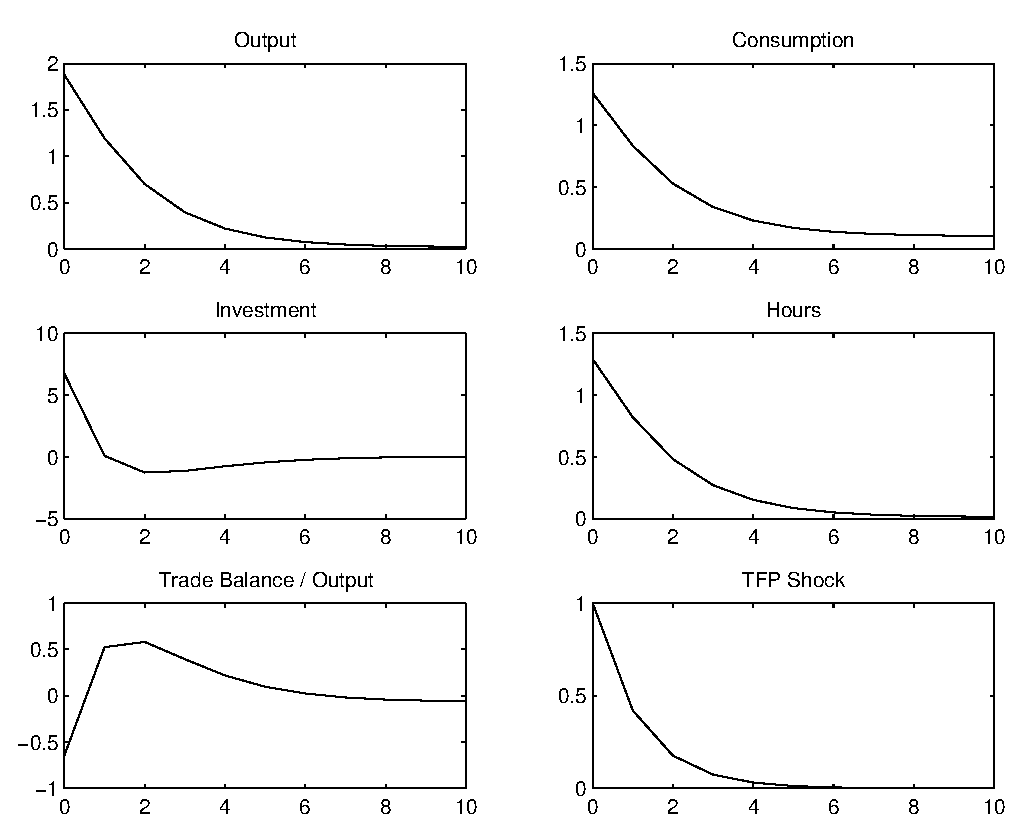
\includegraphics[width = 0.85\linewidth]{FIGURES/soe_rbc_edeir.eps} 

{\tiny Source: Schmitt-Groh\'e and Uribe (JIE, 2003)}

\end{frame}

\section{Comparative Statics of Model}

\begin{frame}
\frametitle{Outline}
\tableofcontents[currentsection]
\end{frame}


\begin{frame}{Response of TB and varying capital adjustment cost}

\begin{center}
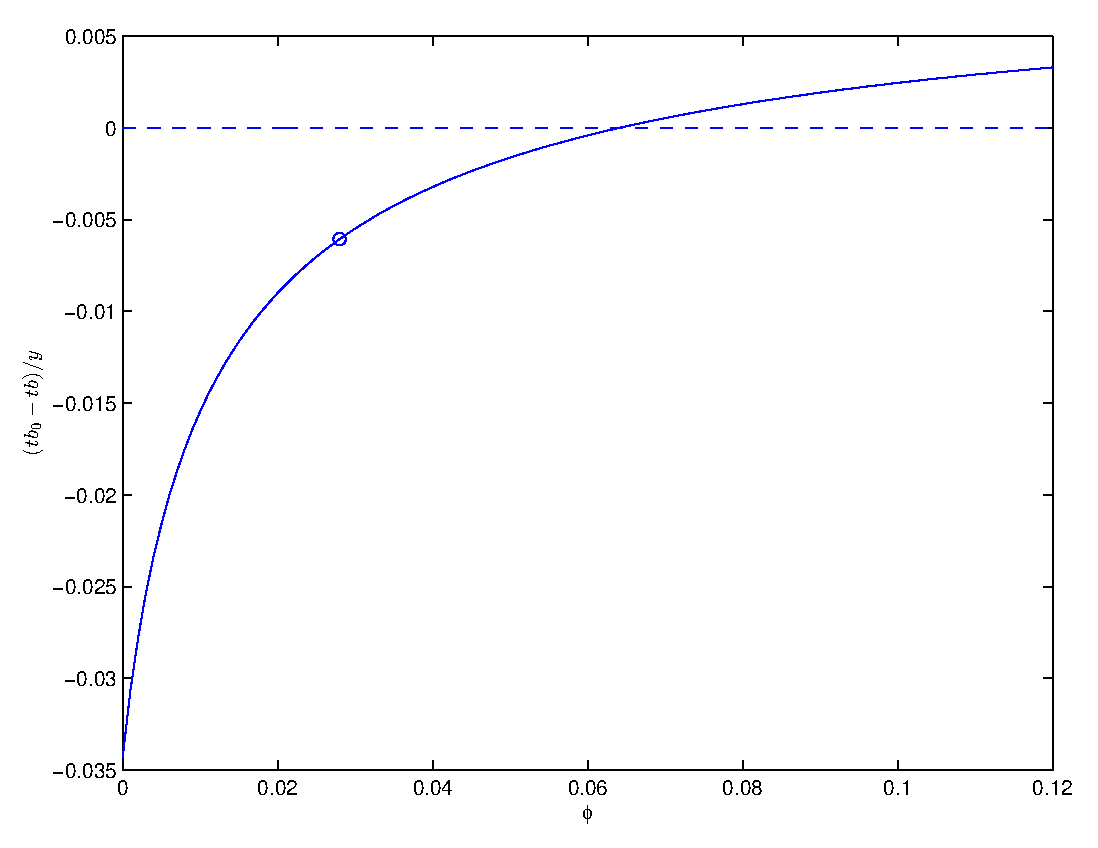
\includegraphics[width = 0.7\linewidth]{FIGURES/soe_rbc_irtbys_phi_slides.eps} 
\end{center}
\vspace{-0.5cm}
%Produced with: Z:\uribe\book\soe_rbc\edeir\edeir_sensitivity\edeir_run.m
Higher capital adj. costs \rarr more positive impulse response of TB. For $\phi<0.06$ (scale parameter of adj. cost), the response of the trade balance negative.
\\
Recall $TB_t = Y_t - C_t - I_t$. With large adj. cost, investment response weak \rarr consumption drives TB \rarr intuition from 2-period model with consumption only applies.

\end{frame}


\begin{frame}{Response of TB and varying productivity persistence}

\begin{center}
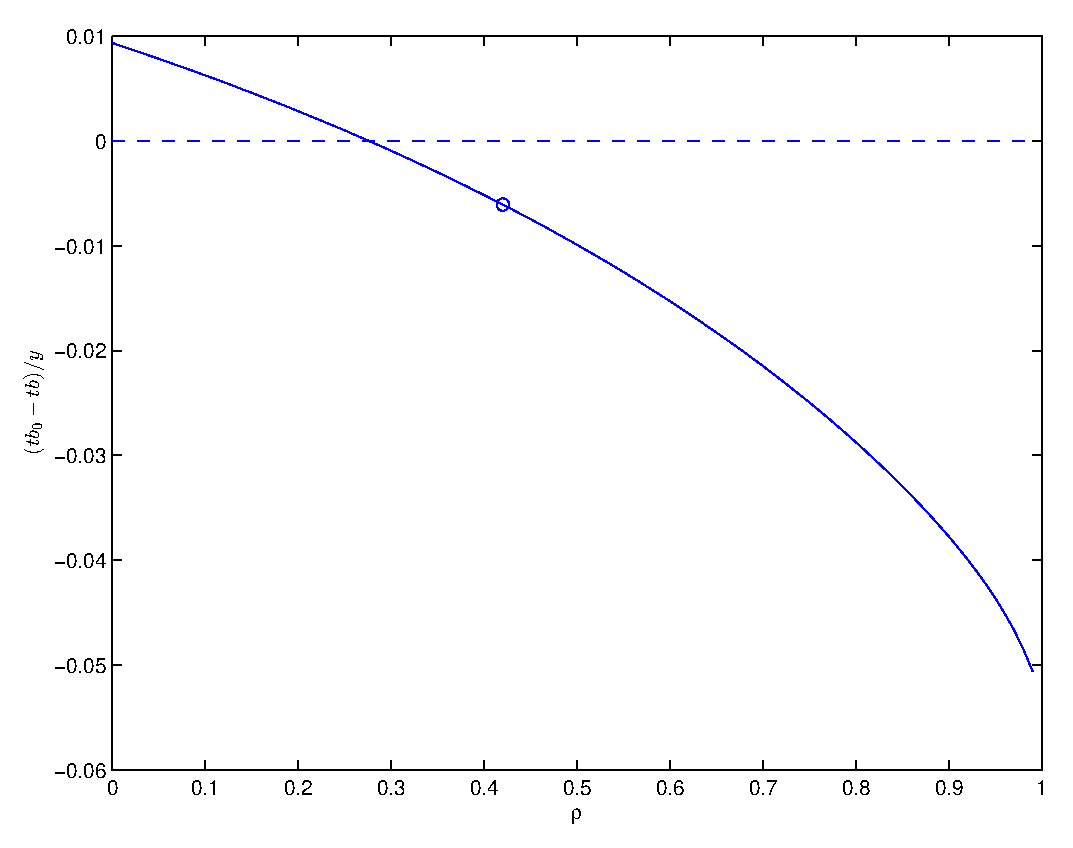
\includegraphics[width = 0.7\linewidth]{FIGURES/soe_rbc_irtbys_rho_slides.eps} 
\end{center}
\vspace{-0.5cm}
%Produced with: Z:\uribe\book\soe_rbc\edeir\edeir_sensitivity\edeir_run.m
More persistent the productivity shock \rarr smaller impulse response of TB (recall temporary vs. permanent shocks in the 2-period model). For $\rho>0.3$ (productivity persistent enough), the response of TB is negative.

\end{frame}
\end{document}
